\documentclass[10pt]{beamer}
\usetheme{Boadilla}

%%% ADD HERE ALL THE PACKAGES YOU USE %%%
% Packages required only for the specific content in this template, remove if not needed
\usepackage{slashed}
\usepackage{dsfont}
\usepackage{amsmath}
\usepackage{amssymb}
\usepackage{bm}


%%% ADD HERE ALL THE PACKAGES YOU USE %%%
% Packages required only for the specific content in this template, remove if not needed
\usepackage{slashed}
\usepackage{dsfont}
\usepackage{amsmath}


%%% COMMANDS & PACKAGES FOR TIKZIT %%%
%%% Requires tikzit.sty in the main folder, remove if not needed
\usepackage{tikzit}
\definecolor{gaugelink}{HTML}{87608b}
\definecolor{plaquette}{HTML}{607b8b}
\input{tikzit/plaquettes.tikzstyles}
% Package needed to scale .tikz diagrams
\usepackage{tikzscale}
\usetikzlibrary{positioning}
\usepackage{multirow}
\usepackage{caption}
\captionsetup[figure]{font=footnotesize}

\usepackage{graphicx}
\usepackage{subcaption}
\captionsetup{compatibility=false}


\usepackage[utf8]{inputenc}
\usepackage[T1]{fontenc}
\usepackage{yfonts}
\usepackage{bm}
\usepackage{amssymb}

\usepackage{verbatim}

%\usepackage{graphicx}
\graphicspath{ {./images/} }
%\usepackage{subfigure}


\usepackage{mathtools}
\usepackage{esint}


\newcommand*{\dd}{\mathop{}\!\mathrm{d}}


\makeatother
\setbeamertemplate{footline}
{
  \leavevmode%
  \hbox{%
  \begin{beamercolorbox}[wd=.4\paperwidth,ht=2.25ex,dp=1ex,center]{author in head/foot}%
    \usebeamerfont{author in head/foot}\insertshortauthor
  \end{beamercolorbox}%
  \begin{beamercolorbox}[wd=.6\paperwidth,ht=2.25ex,dp=1ex,center]{title in head/foot}%
    \usebeamerfont{title in head/foot}\insertshorttitle\hspace*{3em}
    \insertframenumber{} / \inserttotalframenumber\hspace*{1ex}
  \end{beamercolorbox}}%
  \vskip0pt%
}



\makeatletter

\setbeamertemplate{frametitle}{%
  \ifbeamercolorempty[bg]{frametitle}{}{\nointerlineskip}%
  \@tempdima=\textwidth%
  \advance\@tempdima by\beamer@leftmargin%
  \advance\@tempdima by\beamer@rightmargin%
  \begin{beamercolorbox}[sep=0.2cm,left,wd=\the\@tempdima]{frametitle}
    \usebeamerfont{frametitle}%
    \vbox{}\vskip-2ex%
    \if@tempswa\else\csname beamer@fteleft\endcsname\fi%
    \strut\insertframetitle\strut\par%
    {%
      \ifx\insertframesubtitle\@empty%
      \else%
      {\usebeamerfont{framesubtitle}\usebeamercolor[fg]{framesubtitle}\insertframesubtitle\strut\par}%
      \fi
    }%
    \vskip-1ex%
    \if@tempswa\else\vskip-.3cm\fi% set inside beamercolorbox... evil here...
  \end{beamercolorbox}%
}

\setbeamertemplate{navigation symbols}{}


\date{June 30, 2021}
\title{Properties of Seismic Scale-free Networks}
\author{Gabriel Tiberiu Pan\u{a}}
\institute{Theoretical and Computational Physics}

\begin{document}

{
\usebackgroundtemplate{%
\tikz\node[opacity=0.4] {\includegraphics[height=\paperheight,width=\paperwidth]{motifs_romania_5km_4mag_trianglesFilled}};}
\begin{frame}[noframenumbering,plain]
	\titlepage
\end{frame}
}
	
\begin{frame}{Outline}
	\tableofcontents
\end{frame}


\section{Introduction}
\begin{frame}{Introduction}
In this work we will familiarize ourselves with some complexity theory concepts such as complex systems, network theory, critical phenomena and self-organization to criticality.\par

\vspace{5mm} 

Then we will analyze various seismic regions around the globe from the perspective of complex networks with the aid of the mathematical tools of graph theory. We expect that this would reinforce the idea that seismic zones behave as complex, self-organized critical systems.\par 
\end{frame}


\section{Complex Systems}

%{
%\usebackgroundtemplate{%
%\tikz\node[opacity=0.2] {\includegraphics[height=\paperheight,width=\paperwidth]{shoreline}};}
%----------------------------------------------------------------%
\begin{frame}{Complex Systems}

%{\bf Diversity} applies to a collection of entities or a population; it requires a multitude of objects that are to be analyzed. For example, cities, ecosystems, molecular matter, plasma are diverse. When speaking of diversity, we can mean a few different characteristics of a population:
%\begin{itemize}
%	\item {\it variation} of some attribute (eg. difference of height in a group of people).
%	\item {\it diversity} of types (eg. different ethnicities in a social group).
%	\item differences in {\it configuration} (eg. different arrangments in housing units of a group of people).
%\end{itemize} 

{\bf Complexity} can be thought of as particular structures and patterns that cannot be easily described or predicted. A system becomes complex when {\it diverse} rule-following entities behave in an {\it interdependent} way. These entities interact over a {\it contact structure} or {\it network}. Characteristics:
\begin{itemize}
	\item {\it adaptation} (eg. in a social system, individuals can learn, or in an ecosystem natural selection can take place)
	\item {\it robustness} (eg. they exhibit a certain behaviour at any spatio-temporal scale)
	\item {\it large events occurence} (eg. large earthquakes)
	\item {\it equillibrium states, fixed points, patterns or chaotic behaviour}
\end{itemize}

\end{frame}
%}


%----------------------------------------------------------------%
\begin{frame}{Stanley Milgram's Small Worlds}
\begin{figure}[!h]
  \centering
  \includegraphics[width=.5\linewidth]{smallworld}
  \caption{Stanley Milgram's Small Worlds Experiment: A letter randomly sent to a citizen in Nebraska starts on a 6 person's journey to it's target in Boston. Each person mailed the letter to an acquaintance that they thought would be closer to the target. The second to last person, mails the letter to the target because they knew him personally. Image from Elisa Baek et. al., Social Network Analysis for Social Neuroscientists”}
  \label{fig:smallWorld}
\end{figure}
\end{frame}


%----------------------------------------------------------------%
\begin{frame}{Euler's bridges}
Even earlier than Milgram's experiment, the problem that is thought to be the birth of graph theory is the Seven Bridges of Königsberg.\par

\begin{block}{Problem}
Is there a possible walk through the city that would cross each of the seven bridges once and only once?\par 
"No" - Leonhard Euler, 1736
\end{block}

\begin{figure}[!h]
  \centering
  \includegraphics[width=.9\linewidth]{eulerBridges}
  \caption{A depiction of what the problem looks like then and now. On the left, a map of Seventeenth-century Königsberg with the bridges in question highlighted. In the middle, a visualization of how Euler graphically represented the problem and on the right, how we represent the issue today, in modern graph theory. Image credit: Bogdan Giușgă, Wikipedia}
  \label{fig:eulerBridges}
\end{figure}
\end{frame}


%----------------------------------------------------------------%
\begin{frame}
\begin{columns}
          \column{0.28\linewidth}
             \centering
             \includegraphics[width=3.5cm]{eulerBridgeGraph}
           \column{0.68\linewidth}
              \textbf{Euler's Solution}
by walking in the graph, except for the start and finish nodes, one must enter a node as many times as he exists, so the nodes must be touched by even numbers of bridges. This made the connection between walks and node degrees in a graph, meaning that the necessary and sufficient condition for the desired walk is that the graph may have exactly zero or two nodes of odd degree.
         \end{columns} 
         
\vspace{5mm}
         
Since in the problem, all land masses are connected by odd number of bridges, the proposed walk is impossible.\par 

\vspace{5mm}

%Euler's contribution was two-fold: firstly, it is considered to be the first theorem in graph theory and the theory of networks and secondly, the realisation that the information in the problem was the number of bridges and their endpoints represented the beginning of the development of a new area of mathematics named topology.
\end{frame}


%----------------------------------------------------------------%
\begin{frame}{Graph Theory}
Graph theory is the framework for the exact mathematical treatment of complex networks. An undirected (or directed) graph $G=(\mathcal{N},\mathcal{L})$ consists of two sets $\mathcal{N}$ and $\mathcal{L}$:
\begin{itemize}
	\item $\mathcal{N} \equiv \{ n_1,n_2,...,n_N \}$ = the nodes (or vertices, points) of G
	\item $\mathcal{L} \equiv \{ l_1,l_2,...,l_K \}$ = the links (or edges, lines) of G 
\end{itemize}
$G(N,K) = (\mathcal{N},\mathcal{L})$ represents a graph with $N$ nodes and $K$ edges.\par 

\begin{figure}[!h]
  \centering
  \includegraphics[width=.65\linewidth]{graphs}
  \caption{Graphical representation of a few types of graphs, each with $N=7$ nodes and $K=14$ edges: (a) undirected, (b) directed, the arrows showing the direction of each link and (c) weighted undirected, each link's weight $W_{i,j}$ reported on the respective line. Image credit: S. Boccaletti et. al., “Complex networks: Structure and dynamics”}
  \label{fig:graphs}
\end{figure}

\end{frame}

\begin{comment}
%----------------------------------------------------------------%
\begin{frame}
\begin{figure}[!h]
  \centering
  \includegraphics[width=.8\linewidth]{graphs}
  \caption{A few types of graphs, each with $N=7$ nodes and $K=14$ edges: (a) undirected, (b) directed, the arrows showing the direction of each link and (c) weighted undirected, each link's weight $W_{i,j}$ reported on the respective line.}
  \label{fig:graphs}
\end{figure}
\end{frame}


%----------------------------------------------------------------%
\begin{frame}
A few fundamental elements of a graph:
\begin{itemize}
	\item a {\it walk} fom node $i$ to node $j$ = alternating sequence of nodes and edges that begins in $i$ and ends in $j$;
	\item a {\it trail} = a walk in which no edge is repeated;
	\item a {\it path} = a walk in which no node is repeated;
	\item the {\it shortest path} = the walk of minimal length between two nodes;
	\item a {\it cycle} = a closed walk of at least three nodes, usually defined by it's length $k$ or $C_k$ (example: $C_3$ is a triangle, $C_4$ is a quadrilater).
\end{itemize}

Finally a graph is mathematically described by it's {\it adjacency matrix} $\mathcal{A}$, a $N \times N$ matrix whose entries $a_{ij}$ are either $1$ if link $l_{ij}$ exists or $0$ 
otherwise.\par 

\end{frame}

\end{comment}



%\usebackgroundtemplate{%
%\tikz\node[opacity=0.15] {\includegraphics[height=\paperheight,width=\paperwidth]{criticality}};}
%----------------------------------------------------------------%
\begin{frame}{Criticality and Self-organization}

{\bf Critical phenomena} refers to peculiar behaviour of a system when it is near or at the point of a continuous-phase transition, also called a {\it critical} point, which is a point at which the system changes from one state to another without a jump or discontinuity in it's properties such as internal energy, density or magnetization.

\vspace{5mm}

{\bf Self-organization} is the process by which individual components of a system organize their communal behaviour to create global order by interactions amongst themselves rather than through external influence or instruction. Complex dynamic systems which have many and diverse elements interacting with each other, may display features of self-organization. \par
%This phenomena can be triggered by seemingly random fluctuations, amplified by positive feedback.\par 
Fundamental characteristics of this organization are:
\begin{enumerate}
	\item {\bf decentralization} : the organization is distributed over all the components of the system
	\item {\bf robustness} : the system is able to survive or self-repair perturbations
\end{enumerate}
{\bf "In chaos theory, self-organizations represent "islands" of predictability in a sea of chaotic unpredictability".}

\end{frame}




%\usebackgroundtemplate{%
%\tikz\node[opacity=0.35] {\includegraphics[height=\paperheight,width=\paperwidth]{soc}};}
%----------------------------------------------------------------%
\begin{frame}{Self-Organized Criticality}
In his 1996 paper "Simplest Possible Self-Organized Critical System", Flyjberg explains that a SOC system is a driven dissipative system consisting of:
\begin{enumerate}
	\item a {\it medium} which has:
	\item {\it disturbances} propagating through it, causing
	\item a {\it modification} of the medium, such that eventually
	\item the medium is in a {\it critical state} and
	\item the medium is {\it modified no more}
\end{enumerate}
\end{frame}




%\usebackgroundtemplate{%
%\tikz\node[opacity=0.2] {\includegraphics[height=\paperheight,width=\paperwidth]{fractal}};}
%----------------------------------------------------------------%
\begin{frame}
Per Bak, Chao Tang and Kurt Wiesenfeld formulated the followinng key points when they defined Self-Organized Criticality (SOC):
\begin{itemize}
	\item Spatial and temporal scaling must usually be unavoidably connected.
	\item There must be a robust, widespread spatio-temporal critical behaviour which arises from self-organization.
	\item Slow driven interaction and existence of a threshold.
	\item Dissipation has a role in maintaining a SOC state
	%\item Spacetime fractals are snapshots of the SOC state.
\end{itemize}
\end{frame}


\section{Seismic Models}


%----------------------------------------------------------------%
\begin{frame}{Bak, Tang and Wiesenfeld's Sandpile Model}
\begin{figure}[!h]
  \centering
  \includegraphics[width=.5\linewidth]{SOC_sandpile}
  \caption{An illustration from "How Nature Works", a drawing by Elaine Wiesenfeld in which the dropping of grains of sand on a little pile on the beach is pictured.}
  \label{fig:driverBlock}
\end{figure}
\end{frame}

\begin{comment}
%----------------------------------------------------------------%
\begin{frame}
The model is described as a two-dimensional sandpile, a cellular automaton comprising of interactions of an integer variable $z$ (number of sand grains in a site) with it's nearest neighbours. A grid of sites is created, with boundary conditions $z=0$. The sites are updated at random by dropping sand on them, and when $z>K$ (a threshold value) redistribution occurs:
\begin{align}
&z(x,y) \to z(x,y)-4, \\
&z(x\pm 1,y) \to z(x \pm 1,y)+1, \\
&z(x,y\pm 1) \to z(x,y\pm 1)+1.
\end{align}
The site is initiated with random values for each site $z>>K$ and it evolves until it stops $z<K$. \par
Simulations show that the distribution of cluster sizes and time scales follow power-law distributions.\par 
The self-organized critical state of minimally stable clusters is very robust on all length scales and they create fluctuations on all time scales.
\end{frame}
\end{comment}


%----------------------------------------------------------------%
\begin{frame}{Per Bak's Bureaucrats Model}
In his famous book, How Nature Works, Per Bak describes a re-imagination of the sandpile model, called the bureaucrats model. The principle is similar and it is illustrated in the following picture:

\begin{figure}[!h]
  \centering
  \includegraphics[width=.7\linewidth]{SOC_bureaucrats}
  \caption{The "Office" version of the sandpile model. At each timestep a document is placed on the desk of a bureaucrat. When he finds four or more documents on his desk, he redistributes them, one to each of his neighbours, or he throws it out the window if he is at the edge of the room (the boundary conditions).}
  \label{fig:bureaucrats}
\end{figure}
\end{frame}


%----------------------------------------------------------------%
\begin{frame}{Olami-Feder-Christensen Slider-Blocks Model}

\begin{columns}
          \column{0.38\linewidth}
             \centering
             \includegraphics[width=5cm]{SOC_sliderBlocks}
           \column{0.58\linewidth}
              \textbf{The model is constructed as follows :}
               \begin{enumerate}
	\item consider a 2D lattice of blocks;
	\item each block is connected with springs to its four nearest nighbours and to a rigid moving plate;
	\item each block interacts frictionally to a fixed plate that they move on;
	\item blocks are driven by the continuous displacement of the moving plate;
	\item when the force of one of the blocks reaches a threshold value $F_{th}$, the block slips, redefining the forces of it's neighbours;
	
				\end{enumerate}

         \end{columns} 

\vspace{5mm} 

	The slip of one block may result in an avalanche of slips by the nearest blocks resulting in a chain reaction.
\end{frame}


%----------------------------------------------------------------%
\begin{frame}
The model evolves as follows:
\begin{enumerate}
	\item initialize all sites' forces to a random value between 0 and 1;
	\item check if any $F_{ij} \geq F_{th}$;
	\item if yes, redistribute the force according to:
	\begin{align}
	&F_{n,n} \to F_{n,n} + \alpha F_{i,j},\\
	&F_{i,j} \to 0.
	\end{align}
	\item repeat from step 2 until the earthquake fully evolves;
	\item locate the block with $F_{max}$ and add $F_{th}-F_{max}$ to all blocks and return to the second step.
\end{enumerate}
The probability distribution of the total number of relaxations of the slips (earthquakes) is measured. This quantitiy is proportional to the energy release during an earthquake. This cellular automaton model is found to show SOC behaviour for a large number of $\alpha$ values.\par 
\end{frame}


%----------------------------------------------------------------%
\begin{frame}{Slider-blocks model conclusions}
OFC reached the following results with their model:
\begin{itemize}
	\item displays robust SOC behaviour over a number of conservation levels;
	\item the amount of conservation impacts the obtained power-laws;
	\item as conservation increases, the behaviour transitions from localized to nonlocalized;
	\item this conservation dependence explains the variance of the parameter in the Gutenberg-Richter law.
\end{itemize}
\end{frame}
\section{Seismic Databases}


%----------------------------------------------------------------%
\begin{frame}{Seismic Databases}
For each seismic region we wish to study, the first step is to collect the earthquakes databases available online, published by the respective region institute:
\begin{itemize}
	\item {\bf Vrancea(Romania)} - National Institute for Earth Phyiscs.
	\item {\bf California(USA)} - Southern California Earthquake Center.
	\item {\bf Italy} - National Institute for Geophysics and Vulcanology.
	\item {\bf Japan} - Japan Meteorological Agency.
\end{itemize}
\end{frame}


%----------------------------------------------------------------%
\begin{frame}{All data available in databases}
\begin{center}
\centering
 \begin{tabular}{ |c||c|c|c|c|  }

 \hline
 \multicolumn{5}{|c|}{Seismic Databases} \\
 \hline
 Seismic Zone & Timeframe & Latitude & Longitude & Depth\\
 \hline
 \hline
 \multirow{2}{8em}{Romania} & 0984-01-01 & 43.594$^{\circ}$N & 20.1$^{\circ}$E & 0\\
 & 2021-02-28 & 48.23$^{\circ}$N & 26.14$^{\circ}$E & 218.4\\
 \hline
 \multirow{2}{8em}{California(USA)} & 1932-01-02 & 32$^{\circ}$N & -114$^{\circ}$W & 0\\
 & 2020-12-31 & 37$^{\circ}$N & -122$^{\circ}$W & 51.1\\
 \hline
 \multirow{2}{8em}{Italy} & 1986-01-01 & 30.61$^{\circ}$N & -6.08$^{\circ}$W & 0\\
 & 2020-12-31 & 47.998$^{\circ}$N & 36.02$^{\circ}$E & 644.4\\
 \hline
 \multirow{2}{8em}{Japan} & 1919-01-11 & 17.41$^{\circ}$N & 114.78$^{\circ}$E & 0\\
 & 2019-08-31 & 54.97$^{\circ}$N & 160.17$^{\circ}$E & 698.4\\
 \hline
 \end{tabular}
\end{center}
\end{frame}


%----------------------------------------------------------------%
\begin{frame}{Romania and Vrancea} 

\begin{figure}[!h]
\begin{subfigure}{.5\textwidth}
  \centering
  \includegraphics[width=.9\linewidth]{quakesRomania_map}
  \caption{Romania: 29186 earthquakes,\\ from 1976-02-03 13:29:16 to 2021-02-28 16:57:29.}
  \label{fig:sfigRo}
\end{subfigure}%
\begin{subfigure}{.5\textwidth}
  \centering
  \includegraphics[width=.9\linewidth]{quakesVrancea_map}
  \caption{Vrancea: 7512 earthquakes,\\ from 1976-08-19 19:03:01 to 2021-02-28 00:11:55.}
  \label{fig:sfigVrancea}
\end{subfigure}
\caption{Earthquakes distribution for Romania (left) and Vrancea (right) seismic zones with magnitude $>1$.}
\label{fig:simpleScatterRoVr}
\end{figure}

\end{frame}


%----------------------------------------------------------------%
\begin{frame}{California(USA)}
\begin{figure}[!h]
\centering
\includegraphics[width=.5\linewidth]{quakesCalifornia_map}
\caption{Earthquakes distribution for California(USA), seismic zone: 221113 events with magnitude $>1$, from 1984-01-01 18:27:55 to 2020-12-31 23:04:53.}
\label{fig:simpleScatteritaly}
\end{figure}
\end{frame}



%----------------------------------------------------------------%
\begin{frame}{Italy}

\begin{figure}[!h]
\centering
\includegraphics[width=.5\linewidth]{quakesItaly_map}
\caption{Earthquakes distribution for Italy seismic zone: 319567 events with magnitude $>1$, from 1986-01-01 17:22:53 to 2020-12-31 23:41:18.}
\label{fig:simpleScatteritaly}
\end{figure}

\end{frame}


%----------------------------------------------------------------%
\begin{frame}{Japan}
\begin{figure}[!h]
\centering
\includegraphics[width=.5\linewidth]{quakesJapan_map}
\caption{Earthquakes distribution for Japan seismic zone: 595713 events with magnitude $>2$, from 1992-01-01 00:54:03 to 2019-08-31 23:54:24.}
\label{fig:simpleScatterJapan}
\end{figure}
\end{frame}


%----------------------------------------------------------------%
\begin{frame}{Earthquake Table}
The fundamental tool we use in our analysis is the Earthquakes Table:

\begin{figure}[!h]

\centering
\includegraphics[width=\linewidth]{quakesTable}
\caption{The Earthquakes Table - our fundamental tool for the following analysis, containing the basic information from the databases available online ({\it date, latitude, longitude, depth and magnitude}) and our computations: the $energyRelease$ and the "cube parametrization" with indexing both in the "cubes space": $x$, $y$, $z$ and the real space: $cubeLatidue$, $cubeLongitude$, $cubeDepth$.\\ }
\label{fig:quakesTable}
\end{figure}
The data in this example represents the first 5 events in the Vrancea seismic zone, starting with the year 1976, as a pandas DataFrame in Python.

\end{frame}

%----------------------------------------------------------------%
\begin{frame}
\begin{enumerate}
	\item {\bf energyRelease:} we can roughly estimate the energy release of each event by converting the moment magnitude $M_W$ to energy using the equation $log E = 5.24 + 1.44M$ where $M$ is the magnitude. 
	\item {\bf Cube splitting:} in order to build our earthquakes network, we need to divide the spatial region selected into cubes and place each event in it's respective cube.
\end{enumerate}

\begin{figure}[h!]
\centering
\tikz[remember
picture]{\node(1BL){\includegraphics[width=4cm]{quakesVrancea_grid}};}%
\hspace*{3cm}%
\tikz[remember picture]{\node(1BR){\includegraphics[width=4cm]{quakesVrancea_cubeSplit}};}
\end{figure}
\tikz[overlay,remember picture]{\draw[-latex,thick] (1BL) -- (1BL-|1BR.west)
node[midway,below,text width=2cm]{Cube split};} 

\end{frame}


\section{Seismic Networks}


%----------------------------------------------------------------%
\begin{frame}{Graph example of a Seismic Network}

\begin{figure}[h]
\begin{subfigure}[b]{0.4\linewidth}
\centering
\resizebox{0.95\textwidth}{!}{%
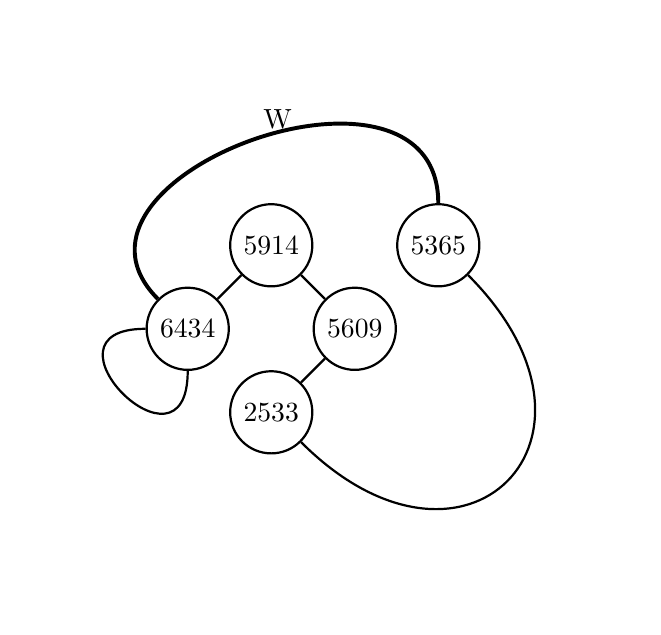
\begin{tikzpicture}[node distance={15mm}, thick, main/.style = {draw, circle}] 
\node[main] (1) {$6434$}; 
\node[main] (2) [above right of=1] {$5914$}; 
\node[main] (3) [below right of=1] {$2533$}; 
\node[main] (4) [above right of=3] {$5609$}; 
\node[main] (5) [above right of=4] {$5365$}; 

\draw(1) -- (2); 
%\draw(1) -- (3); 
\draw [line width=0.05cm] (1) to [out=135,in=90,looseness=1.5] node[midway, above right] {W}  (5); 
\draw (1) to [out=180,in=270,looseness=5] (1); 
\draw (2) -- (4); 
\draw (3) -- (4); 
%\draw (5) -- (4); 
\draw (5) to [out=315, in=315, looseness=2.5]  (3); 
\end{tikzpicture}}
\end{subfigure}
\begin{subfigure}[b]{0.4\linewidth}
  \includegraphics[width=\textwidth]{quakesTable2}
  \label{fig:qTab2}
\end{subfigure}%

\caption{Seismic Network (Graph representation) example: Nodes are identified as $cubeIndex$, used to acces any information about events in that respective cube from our Earthquakes Table. Edge weight can be represented on the edge as $W$, where each additional link between two nodes increases this value by 1.}
\end{figure}

\end{frame}


%----------------------------------------------------------------%
\begin{frame}{Connectivity of a Network}
The fundamental measure to describe our seismic network is the connectivity distribution $P(k)$. This distribution comes naturally by realising the histogram of the nodes degree and then the regression of the distribution and show that it follows a power law:

\begin{equation}
P(k) \sim k^{-\gamma}
\end{equation}

The connectivity computations are made for various seismic networks (Vrancea(Romania), California(USA), Italy and Japan), with different magnitude restrictions, for 2 cube sizes: $5\times5\times5$ km and $10\times10\times10$ km, with and without edge weights.
\end{frame}


% ---------------------------- VRANCEA CONNECTIVITY ----------------------------%
%----------------------------------------------------------------%
\begin{frame}{Vrancea Connectivity}
\begin{figure}[!h]
\begin{subfigure}{.5\textwidth}
  \includegraphics[width=\textwidth]{connectivityVrancea_1magnitude10}
  \caption{$1 \leq magnitude$}
  \label{fig:conVr1mag10}
\end{subfigure}%
\hfill
\begin{subfigure}{.5\textwidth}
  \includegraphics[width=\textwidth]{connectivityVrancea_2magnitude10}
  \caption{$2 \leq magnitude$}
  \label{fig:conVr2mag10}
\end{subfigure}%

\vskip\baselineskip

\begin{subfigure}{.5\textwidth}
  \includegraphics[width=\textwidth]{connectivityVrancea_2magnitude4}
  \caption{$2\leq magnitude \leq 4$}
  \label{fig:conVr2mag14}
\end{subfigure}%
\hfill
\begin{subfigure}{.5\textwidth}
  \includegraphics[width=\textwidth]{connectivityVrancea_3magnitude7}
  \caption{$3 \leq magnitude \leq 7$}
  \label{fig:conVr3mag7}
\end{subfigure}%

\caption{Connectivity distribution $P(k)$ for Vrancea in log-log and interpolation of the results, for a number of magnitude ranges. The exponent of the power law, $\gamma$ ranges from $\sim 1.08$ to $1.756$.}
\label{fig:connectivityVr}
\end{figure}
\end{frame}


%----------------------------------------------------------------%
\begin{frame}{Vrancea Weighted Connectivity}
\begin{figure}[!h]
\begin{subfigure}{.5\textwidth}
  \includegraphics[width=\columnwidth]{connectivityVranceaWeighted_1magnitude10}
  \caption{$1 \leq magnitude$}
  \label{fig:conWeiVr1mag10}
\end{subfigure}%
\hfill
\begin{subfigure}{.5\textwidth}
  \includegraphics[width=\columnwidth]{connectivityVranceaWeighted_2magnitude10}
  \caption{$2 \leq magnitude$}
  \label{fig:conWeiVr2mag10}
\end{subfigure}%

\vskip\baselineskip

\begin{subfigure}{.5\textwidth}
  \includegraphics[width=\columnwidth]{connectivityVranceaWeighted_2magnitude4}
  \caption{$2\leq magnitude \leq 4$}
  \label{fig:conWeiVr2mag4}
\end{subfigure}%
\hfill
\begin{subfigure}{.5\textwidth}
  \includegraphics[width=\columnwidth]{connectivityVranceaWeighted_3magnitude7}
  \caption{$3 \leq magnitude \leq 7$}
  \label{fig:conWeiVr3mag7}
\end{subfigure}%

\caption{Weighted connectivity distribution $P(k)$ for Vrancea in log-log and interpolation of the results, for a number of magnitude ranges. The exponent of the power law, $\gamma$ ranges from $\sim 1.95$ to $3.26$.}
\label{fig:connectivityVrWeighted}
\end{figure}
\end{frame}


% ---------------------------- California CONNECTIVITY ----------------------------%
%----------------------------------------------------------------%
\begin{frame}{California Connectivity}
\begin{figure}[!h]
\begin{subfigure}{.5\textwidth}
  \includegraphics[width=\columnwidth]{connectivityCalifornia_1magnitude10}
  \caption{$1 \leq magnitude$}
  \label{fig:conCa1mag10}
\end{subfigure}%
\hfill
\begin{subfigure}{.5\textwidth}
  \includegraphics[width=\columnwidth]{connectivityCalifornia_2magnitude10}
  \caption{$2\leq magnitude$}
  \label{fig:conCa2mag10}
\end{subfigure}%

\vskip\baselineskip

\begin{subfigure}{.5\textwidth}
  \includegraphics[width=\columnwidth]{connectivityCalifornia_1magnitude3}
  \caption{$1 \leq magnitude \leq 3$}
  \label{fig:conCa1mag3}
\end{subfigure}%
\hfill
\begin{subfigure}{.5\textwidth}
  \centering
  \includegraphics[width=\columnwidth]{connectivityCalifornia_2magnitude4}
  \caption{$2 \leq magnitude \leq 4$}
  \label{fig:conCa2mag4}
\end{subfigure}%

\caption{Connectivity distribution $P(k)$ for California in log-log and interpolation of the results, for a number of magnitude ranges. The exponent of the power law, $\gamma$ ranges from $\sim 1.45$ to $2.16$.}
\label{fig:connectivityCa}
\end{figure}
\end{frame}


%----------------------------------------------------------------%
\begin{frame}{California - Connectivity Weighted}
\begin{figure}[!h]
\begin{subfigure}{.5\textwidth}
  \includegraphics[width=\columnwidth]{connectivityCaliforniaWeighted_1magnitude10}
  \caption{$1 \leq magnitude$}
  \label{fig:conWeiCa1mag10}
\end{subfigure}%
\hfill
\begin{subfigure}{.5\textwidth}
  \includegraphics[width=\columnwidth]{connectivityCaliforniaWeighted_2magnitude10}
  \caption{$2\leq magnitude$}
  \label{fig:conWeiCa2mag10}
\end{subfigure}%

\vskip\baselineskip

\begin{subfigure}{.5\textwidth}
  \includegraphics[width=\columnwidth]{connectivityCaliforniaWeighted_1magnitude3}
  \caption{$1 \leq magnitude \leq 3$}
  \label{fig:conWeiCa1mag3}
\end{subfigure}%
\hfill
\begin{subfigure}{.5\textwidth}
  \includegraphics[width=\columnwidth]{connectivityCaliforniaWeighted_2magnitude4}
  \caption{$2 \leq magnitude \leq 4$}
  \label{fig:conWeiCa2mag4}
\end{subfigure}%

\caption{Weighted connectivity distribution $P(k)$ for California in log-log and interpolation of the results, for a number of magnitude ranges. The exponent of the power law, $\gamma$ ranges from $\sim 2.06$ to $2.71$.}
\label{fig:connectivityCaWeighted}
\end{figure}
\end{frame}


% ---------------------------- Italy CONNECTIVITY ----------------------------%
%----------------------------------------------------------------%
\begin{frame}{Italy - Connectivity}
\begin{figure}[!h]
\begin{subfigure}{.5\textwidth}
  \includegraphics[width=\columnwidth]{connectivityItaly_1magnitude10}
  \caption{$1 \leq magnitude$}
  \label{fig:conIt1mag10}
\end{subfigure}%
\hfill
\begin{subfigure}{.5\textwidth}
  \includegraphics[width=\columnwidth]{connectivityItaly_2magnitude10}
  \caption{$2\leq magnitude$}
  \label{fig:conIt2mag10}
\end{subfigure}%

\vskip\baselineskip

\begin{subfigure}{.5\textwidth}
  \includegraphics[width=\columnwidth]{connectivityItaly_1magnitude3}
  \caption{$1 \leq magnitude \leq 3$}
  \label{fig:conIt1mag3}
\end{subfigure}%
\hfill
\begin{subfigure}{.5\textwidth}
  \includegraphics[width=\columnwidth]{connectivityItaly_2magnitude4}
  \caption{$2 \leq magnitude \leq 4$}
  \label{fig:conIt2mag4}
\end{subfigure}%

\caption{Connectivity distribution $P(k)$ for Italy in log-log and interpolation of the results, for a number of magnitude ranges. The exponent of the power law, $\gamma$ ranges from $\sim 1.44$ to $2.3$.}
\label{fig:connectivityIt}
\end{figure}
\end{frame}


%----------------------------------------------------------------%
\begin{frame}{Italy - Connectivity Weighted}
\begin{figure}[!h]
\begin{subfigure}{.5\textwidth}
  \includegraphics[width=\columnwidth]{connectivityItalyWeighted_1magnitude10}
  \caption{$1 \leq magnitude$}
  \label{fig:conWeiIt1mag10}
\end{subfigure}%
\hfill
\begin{subfigure}{.5\textwidth}
  \centering
  \includegraphics[width=\columnwidth]{connectivityItalyWeighted_2magnitude10}
  \caption{$1 \leq magnitude$}
  \label{fig:conWeiIt2mag10}
\end{subfigure}%

\vskip\baselineskip

\begin{subfigure}{.5\textwidth}
  \includegraphics[width=\columnwidth]{connectivityItalyWeighted_1magnitude3}
  \caption{$1 \leq magnitude \leq 3$}
  \label{fig:conWeiIt1mag3}
\end{subfigure}%
\hfill
\begin{subfigure}{.5\textwidth}
  \includegraphics[width=\columnwidth]{connectivityItalyWeighted_2magnitude4}
  \caption{$2 \leq magnitude \leq 4$}
  \label{fig:conWeiIt2mag4}
\end{subfigure}%

\caption{Weighted connectivity distribution $P(k)$ for Italy in log-log and interpolation of the results, for a number of magnitude ranges. The exponent of the power law, $\gamma$ ranges from $\sim 2.8$ to $3.72$.}
\label{fig:connectivityItWeighted}
\end{figure}
\end{frame}


% ---------------------------- Japan CONNECTIVITY ----------------------------%
%----------------------------------------------------------------%
\begin{frame}{Japan - Connectivity}
\begin{figure}[!h]
\begin{subfigure}{.5\textwidth}
  \includegraphics[width=\columnwidth]{connectivityJapan_1magnitude10}
  \caption{$1 \leq magnitude$}
  \label{fig:conJa1mag10}
\end{subfigure}%
\hfill
\begin{subfigure}{.5\textwidth}
  \includegraphics[width=\columnwidth]{connectivityJapan_2magnitude10}
  \caption{$2\leq magnitude$}
  \label{fig:conJa2mag10}
\end{subfigure}%

\vskip\baselineskip

\begin{subfigure}{.5\textwidth}
  \includegraphics[width=\columnwidth]{connectivityJapan_1magnitude3}
  \caption{$1 \leq magnitude \leq 3$}
  \label{fig:conJa1mag3}
\end{subfigure}%
\hfill
\begin{subfigure}{.5\textwidth}
  \includegraphics[width=\columnwidth]{connectivityJapan_2magnitude4}
  \caption{$2 \leq magnitude \leq 4$}
  \label{fig:conJa2mag4}
\end{subfigure}%

\caption{Connectivity distribution $P(k)$ for Japan in log-log and interpolation of the results, for a number of magnitude ranges. The exponent of the power law, $\gamma$ ranges from $\sim 1.87$ to $2.5$.}
\label{fig:connectivityJa}
\end{figure}
\end{frame}


%----------------------------------------------------------------%
\begin{frame}{Japan - Connectivity Weighted}
\begin{figure}[!h]
\begin{subfigure}{.5\textwidth}
  \includegraphics[width=\columnwidth]{connectivityJapanWeighted_1magnitude10}
  \caption{$1 \leq magnitude$}
  \label{fig:conWeiJa1mag10}
\end{subfigure}%
\hfill
\begin{subfigure}{.5\textwidth}
  \centering
  \includegraphics[width=\columnwidth]{connectivityJapanWeighted_2magnitude10}
  \caption{$2\leq magnitude$}
  \label{fig:conWeiJa2mag10}
\end{subfigure}%

\vskip\baselineskip

\begin{subfigure}{.5\textwidth}
  \includegraphics[width=\columnwidth]{connectivityJapanWeighted_1magnitude3}
  \caption{$1\leq magnitude \leq 3$}
  \label{fig:conWeiJa1mag3}
\end{subfigure}%
\hfill
\begin{subfigure}{.5\textwidth}
  \includegraphics[width=\columnwidth]{connectivityJapanWeighted_2magnitude4}
  \caption{$2 \leq magnitude \leq 4$}
  \label{fig:conWeiJa2mag4}
\end{subfigure}%

\caption{Weighted connectivity distribution $P(k)$ for Japan in log-log and interpolation of the results, for a number of magnitude ranges. The exponent of the power law, $\gamma$ ranges from $\sim 2.45$ to $3.17$.}
\label{fig:connectivityItWeighted}
\end{figure}
\end{frame}


%----------------------------------------------------------------%
\begin{frame}{Motifs}
Network motifs are sub-graphs that repeat themselves in a specific network or even among various networks. Each of these sub-graphs, defined by a particular pattern of interactions between vertices, may reflect a framework in which particular functions are achieved efficiently.

\begin{figure}
\centering
\includegraphics[width=.6\columnwidth]{4nodeMotifs}
\caption{All 6 possible connected planar 4-node motifs. The most basic of them, the square, would outline a tetrahedron in 3D space}
\end{figure}
\end{frame}


%----------------------------------------------------------------%
\begin{frame}
Given an undirected graph $G=(\mathcal{N},\mathcal{L})$ and any possible small connected graph $F_{n,l}$ with $n$ nodes and $l$ links, we wish to find if $F$ is a significant subgraph of $G$. \\
%This is done by comparing the number of subgraphs of $G$ isomorphic to $F$ with the number of subraphs of a randomised network $G'=(\mathcal{N},\mathcal{L})$ isomorphic to $F$.\\
The simplest approach to quantify the relevance of $F_{n,l}$ as a subgraph of $G$ is based on the evaluation of the {\it Z-score}, defined as follows:
\begin{equation}
Z_F = \frac{n_f - \bar{n}^{rand}_F}{\sigma_{n_F}^{rand}}
\end{equation}
where $n_F$ is the number of times the subgraph $F_{n,l}$ appears in $G$ and $\bar{n}^{rand}_F$ and $\sigma_{n_F}^{rand}$ are the mean and the standard deviation, respectively, of the number of occurences in an ensemble of graphs obtained by randomising $G$.\par 
\end{frame}


%----------------------------------------------------------------%
\begin{frame}{NemoSuite}
\begin{columns}
          \column{0.38\linewidth}
             \centering
             \includegraphics[width=4.4cm]{nemo}
           \column{0.58\linewidth}
              \textbf{NemoSuite (Network Motif Analysis in a Suite)}
                is a web program developed and hosted online by researchers at University of Washington Bothell CSSE to detect and analyze network motifs.\par 
                \vspace{5mm}
                
                A network motif is a frequent and unique subgraph
pattern in an input network, and it is determined by Z-score being larger than $2$.
                
	
         \end{columns} 

\end{frame}


%----------------------------------------------------------------%
\begin{frame}{Triangle Surfaces}
Our goal is to identify motifs in our networks and compute the distribution of their areas weighted by the total and mean energy that is released by earthquakes contained in them.\par 

\vspace{5mm} 

The 3 nodes motifs in 3D space (as in 2D) they outline {\it triangles}. Calculations proceed as follows:
\begin{itemize}
	\item Use NemoSuite to extract all the triangles;
	\item Calculate mean energy and total energy in each motif;
	\item Calculate the total surface of each motif, using the coordinates of the nodes;
	\item Compute the distribution of surfaces weighted by mean/total energy;
	\item Compute the regression using a power-law and find $gamma$ exponent. 
\end{itemize}
\end{frame}

% ---------------------- VRANCEA TRIANGLES -------------------
%----------------------------------------------------------------%
\begin{frame}{Vrancea Mean Energy Weighted Surfaces}
\begin{figure}[h!]
\begin{subfigure}{.5\textwidth}
  \includegraphics[width=\columnwidth]{quakesVrancea_meanEnergy_1mag_trianglesAreas}
  \caption{$1 \leq magnitude$}
  \label{fig:trianglesVrME1}
\end{subfigure}%
\hfill
\begin{subfigure}{.5\textwidth}
  \includegraphics[width=\columnwidth]{quakesVrancea_meanEnergy_2mag_trianglesAreas}
  \caption{$2 \leq magnitude$}
  \label{fig:trianglesVrME2}
\end{subfigure}%

\vskip\baselineskip

\begin{subfigure}{.5\textwidth}
  \centering
  \includegraphics[width=\columnwidth]{quakesVrancea_meanEnergy_3mag_trianglesAreas}
  \caption{$3 \leq magnitude$}
  \label{fig:trianglesVrME3}
\end{subfigure}%

\caption{$S_{ME} = Surface/Mean$ $Energy$ distribution in log-log plots for triangle motifs in Vrancea for 3 magnitude restrictions. The resulting interpolation shows that the distribution appears scale-free with $\gamma$ ranging from $\sim 1.14$ to $2.1$ }
\label{fig:trianglesSurfacesVrME}
\end{figure}
\end{frame}


%----------------------------------------------------------------%
\begin{frame}{Vrancea - Total Energy Weighted Surfaces}
\begin{figure}[h!]

\begin{subfigure}{.5\textwidth}
  \includegraphics[width=\columnwidth]{quakesVrancea_totalEnergy_1mag_trianglesAreas}
  \caption{$1 \leq magnitude$}
  \label{fig:trianglesVrTE1}
\end{subfigure}%
\hfill
\begin{subfigure}{.5\textwidth}
  \centering
  \includegraphics[width=\columnwidth]{quakesVrancea_totalEnergy_2mag_trianglesAreas}
  \caption{$2 \leq magnitude$}
  \label{fig:trianglesVrTE2}
\end{subfigure}%

\vskip\baselineskip

\begin{subfigure}{.5\textwidth}
  \centering
  \includegraphics[width=\columnwidth]{quakesVrancea_totalEnergy_3mag_trianglesAreas}
  \caption{$3 \leq magnitude$}
  \label{fig:trianglesVrTe3}
\end{subfigure}%

\caption{$S_{TE} = Surface/Total$ $Energy$ distribution in log-log plots for triangle motifs in Vrancea for 3 magnitude restrictions. The resulting interpolation shows that the distribution appears scale-free with $\gamma$ ranging from $\sim 2.79$ to $3.67$ }
\label{fig:trianglesSurfacesVrTE}
\end{figure}
\end{frame}


% ---------------------- CALIFORNIA TRIANGLES -------------------____%
%----------------------------------------------------------------%
\begin{frame}{California - Mean Energy Weighted Surfaces}
\begin{figure}[h!]

\begin{subfigure}{.99\textwidth}
  \centering
  \includegraphics[width=.6\columnwidth]{quakesCalifornia_meanEnergy_2mag_trianglesAreas}
  \caption{$2 \leq magnitude$}
  \label{fig:trianglesCaME2}
\end{subfigure}%

\begin{subfigure}{.99\textwidth}
  \centering
  \includegraphics[width=.6\columnwidth]{quakesCalifornia_meanEnergy_3mag_trianglesAreas}
  \caption{$3 \leq magnitude$}
  \label{fig:trianglesCaME3}
\end{subfigure}%

\caption{$S_{ME} = Surface/Mean$ $Energy$ distribution in log-log plots for triangle motifs in California for 2 magnitude restrictions. The resulting interpolation shows that the distribution appears scale-free with $\gamma$ ranging from $\sim 1.42$ to $4.46$}
\label{fig:trianglesSurfacesCaME}
\end{figure}

\end{frame}


%----------------------------------------------------------------%
\begin{frame}{California - Total Energy Weighted Surfaces}
\begin{figure}[h!]

\begin{subfigure}{.99\textwidth}
  \centering
  \includegraphics[width=.6\columnwidth]{quakesCalifornia_totalEnergy_2mag_trianglesAreas}
  \caption{$2 \leq magnitude$}
  \label{fig:trianglesCaTE2}
\end{subfigure}%

\begin{subfigure}{.99\textwidth}
  \centering
  \includegraphics[width=.6\columnwidth]{quakesCalifornia_totalEnergy_3mag_trianglesAreas}
  \caption{$3 \leq magnitude$}
  \label{fig:trianglesCaTe3}
\end{subfigure}%

\caption{$S_{TE} = Surface/Total$ $Energy$ distribution in log-log plots for triangle motifs in California for 2 magnitude restrictions. The resulting interpolation shows that the distribution appears scale-free with $\gamma$ ranging from $\sim 2.56$ to $5.01$ }
\label{fig:trianglesSurfacesCaTE}
\end{figure}
\end{frame}


% ---------------------- Italy TRIANGLES -------------------____%
%----------------------------------------------------------------%
\begin{frame}{Italy - Mean Energy Weighted Surfaces}

\begin{figure}[h!]
  \centering
  \includegraphics[width=.85\columnwidth]{quakesItaly_meanEnergy_2mag_trianglesAreas}
  \label{fig:trianglesItME2}
\caption{$S_{ME} = Surface/Mean$ $Energy$ distribution in log-log plots for triangle motifs in Italy for $2 \leq magnitude$. The resulting interpolation shows that the distribution appears scale-free better at 10 km cube side granularization, with $\gamma = 1.503$ }
\label{fig:trianglesSurfacesItME}
\end{figure}
\end{frame}

%----------------------------------------------------------------%
\begin{frame}{Tetrahedrons Volumes}
Our goal is to identify motifs in our networks and compute the distribution of their volumes weighted by the total and mean energy that is released by earthquakes contained in them.\par 

\vspace{5mm} 

The 4 nodes motifs in 3D space they outline {\it tetrahedrons}. Calculations proceed as follows:
\begin{itemize}
	\item Use NemoSuite to extract all the tetrahedrons;
	\item Calculate mean energy and total energy in each motif;
	\item Calculate the total volume of each motif, using the coordinates of the nodes;
	\item Compute the distribution of volumes weighted by mean/total energy;
	\item Compute the regression using a power-law and find $gamma$ exponent. 
\end{itemize}
\end{frame}


%------------%-----------VRANCEA SQUARES ---------------%
%----------------------------------------------------------------%
\begin{frame}{Vrancea Mean Energy Weighted Volumes}
\begin{figure}[!h]
\begin{subfigure}{.5\textwidth}
  \includegraphics[width=\columnwidth]{quakesVrancea_meanEnergy_1mag_squaresVolumes}
  \caption{$1 \leq magnitude$}
  \label{fig:volumesVrME1}
\end{subfigure}%
\hfill
\begin{subfigure}{.5\textwidth}
  \includegraphics[width=\columnwidth]{quakesVrancea_meanEnergy_2mag_squaresVolumes}
  \caption{$2 \leq magnitude$}
  \label{fig:volumesVrME2}
\end{subfigure}%

\vskip\baselineskip

\begin{subfigure}{.5\textwidth}
  \centering
  \includegraphics[width=\columnwidth]{quakesVrancea_meanEnergy_3mag_squaresVolumes}
  \caption{$3 \leq magnitude$}
  \label{fig:volumesVrME3}
\end{subfigure}%

\caption{$V_{ME} = Volume/Mean$ $Energy$ distribution in log-log plots for tetrahedron motifs in Vrancea for 3 magnitude restrictions. The resulting interpolation shows that the distribution appears scale-free with $\gamma$ ranging from $\sim 1.44$ to $2.8$}
\label{fig:tetrahedronsVolumesVrME}
\end{figure}
\end{frame}


%----------------------------------------------------------------%
\begin{frame}{Vrancea Total Energy Weighted Volumes}
\begin{figure}[!h]
\begin{subfigure}{.5\textwidth}
  \includegraphics[width=\columnwidth]{quakesVrancea_totalEnergy_1mag_squaresVolumes}
  \caption{$1 \leq magnitude$}
  \label{fig:volumesVrTE1}
\end{subfigure}%
\hfill
\begin{subfigure}{.5\textwidth}
  \includegraphics[width=\columnwidth]{quakesVrancea_totalEnergy_2mag_squaresVolumes}
  \caption{$2 \leq magnitude$}
  \label{fig:volumesVrTE2}
\end{subfigure}%

\vskip\baselineskip

\begin{subfigure}{.5\textwidth}
  \centering
  \includegraphics[width=\columnwidth]{quakesVrancea_totalEnergy_3mag_squaresVolumes}
  \caption{$3 \leq magnitude$}
  \label{fig:volumesVrTE3}
\end{subfigure}%

\caption{$V_{TE} = Volume/Total$ $Energy$ distribution in log-log plots for tetrahedron motifs in Vrancea for 3 magnitude restrictions. The resulting interpolation shows that the distribution appears scale-free with $\gamma$ ranging from $\sim 2.94$ to $4.77$}
\label{fig:tetrahedronsVolumesVrTE}
\end{figure}
\end{frame}


%------------%----------- CALIFORNIA SQUARES ---------------%
%----------------------------------------------------------------%
\begin{frame}{California - Mean Energy Weighted Volumes}

\begin{figure}[!h]
  \centering
  \includegraphics[width=.85\columnwidth]{quakesCalifornia_meanEnergy_3mag_squaresVolumes}

\caption{$V_{ME} = Volume/Mean$ $Energy$ distribution in log-log plots for tetrahedron motifs in California for $3 \leq magnitude$. The resulting interpolation shows that the distribution appears scale-free better at 10 km cube side granularization, with $\gamma = 1.835$}
\label{fig:tetrahedronsVolumesCaME}
\end{figure}

\end{frame}


%------------%----------- Italy SQUARES ---------------%
%----------------------------------------------------------------%
\begin{frame}{Italy - Mean Energy Weighted Volumes}
\begin{figure}[!h]
  \centering
  \includegraphics[width=.85\columnwidth]{quakesItaly_meanEnergy_3mag_squaresVolumes}
\caption{$V_{ME} = Volume/Mean$ $Energy$ distribution in log-log plots for tetrahedron motifs in Italy for $3 \leq magnitude$. The resulting interpolation shows that the distribution appears scale-free  better at 10 km cube side granularization, with $\gamma = 3.371$}
\label{fig:tetrahedronsVolumesItME}
\end{figure}
\end{frame}


% --------------------------- MOTIFS IN PARAVIEW -------------------------%
%----------------------------------------------------------------%
{
\usebackgroundtemplate{%
\tikz\node[opacity=0.55] {\includegraphics[height=\paperheight,width=\paperwidth]{paraview}};}
\begin{frame}{Motifs Visualization in Paraview}
As a visualization tool for the earthquakes networks and their motifs we used the application ParaView, which works together with the python library "VTK".\par

\vspace{5mm}

{\bf The Visualization ToolKit (VTK)} is an open source software system for 3D graphics, visualization and image processing. VTK supports a variety of visualization algorithms : scalar, vector, tensor, texture and volumetric methods, making it easy to translate graphs into geometric form.\par

\vspace{5mm}

{\bf ParaView} is an open-source application designed to visualize data of varying sizes, from small to very large. Under the hood, ParaView uses VTK as the data processing and rendering engine.\par 
\end{frame}
}



%----------------------------------------------------------------%
\begin{frame}{Romania - Real Network Visualization}
\begin{figure}[!h]
  \centering
  \includegraphics[width=.85\linewidth]{motifs_romania_5km_4mag_trianglesFilled}
  \caption{Motifs in Romania Seismic Network, earthquakes with magnitude $>4$. Most of the network is concentrated in the Vrancea seismic zone.}
  \label{fig:motifRomania}
\end{figure}
\end{frame}


%----------------------------------------------------------------%
\begin{frame}{Vrancea - Real Network Visualization}
\begin{figure}[!h]
\begin{subfigure}{.5\textwidth}
  \centering
  \includegraphics[width=.85\linewidth]{motifs_vrancea_5km_4mag_trianglesFilled_map}
  \caption{Triangles in Vrancea Seismic Network}
  \label{fig:motifTriangleVrancea}
\end{subfigure}%
\begin{subfigure}{.5\textwidth}
  \centering
  \includegraphics[width=.85\linewidth]{motifs_vrancea_5km_4mag_squaresFilled_map}
  \caption{Tetrahedrons in Vrancea Seismic Network}
  \label{fig:motifTetrahedronVrancea}
\end{subfigure}
\caption{Motifs in Vrancea Seismic Network - 380 events stored in 255 nodes and connected through 375 edges. The degree of connectivity of the nodes ranges from 1 to 16. The motifs are represented as surfaces, for the triangles, or by volumes for the tetrahedrons (drawn in red)}
\label{fig:volumesVrancea}
\end{figure}
\end{frame}


%----------------------------------------------------------------%
\begin{frame}{California - Real Network Visualization}
\begin{figure}[!h]
  \centering
  \includegraphics[width=.85\linewidth]{motifs_california_5km_4mag_trianglesFilled_map}
  \caption{Triangle motifs in California Seismic Network, earthquakes with magnitude $>4$ : 1119 events are stored in 718 nodes, which are connected by 1036 edges.}
  \label{fig:motifCalifornia}
\end{figure}
\end{frame}


%----------------------------------------------------------------%
\begin{frame}{Italy - Real Network Visualization}
\begin{figure}[!h]
  \centering
  \includegraphics[width=.85\linewidth]{motifs_italy_5km_4mag_squaresFilled}
  \caption{Tetrahedron motifs in Italy Seismic Network, earthquakes with magnitude $>4$ : 1490 events are stored in 1325 nodes, which are connected by 1452 edges.}
  \label{fig:motifItaly}
\end{figure}
\end{frame}


%----------------------------------------------------------------%
\begin{frame}{Japan - Real Network Visualization}
\begin{figure}[!h]
  \centering
  \includegraphics[width=.85\linewidth]{motifs_japan_5km_5mag_triangles}
  \caption{Triangle motifs in Japan Seismic Network, earthquakes with magnitude $>5$ : 16948 events are stored in 14396 nodes, which are connected by 20332 edges.}
  \label{fig:motifJapan}
\end{figure}
\end{frame}



\section{Autocorrelations}


%----------------------------------------------------------------%
\begin{frame}{Correlations and Autocorrelations}
Correlations represent a measure of how one value or system responds to another. There are many different types of correlation functions which can be used to determine the correlation of two random variables or systems. For example, time correlation functions are used in the theory of noise and stochastic processes in statistical physics and spectroscopy. \par 

Two types of correlation:
\begin{enumerate}
	\item {\bf cross-correlation} - when two {\bf different} sequences are correlated (eg. comparing two different time series, allowing to see how two signals match )
	\item {\bf autocorrelation} - the correlation occurs between two of the {\bf same} sequences (i.e you correlate the signal with itself).
\end{enumerate}
\end{frame}


\begin{comment}
%--------------------------SPATIAL AUTOCORR -----------------------%
%----------------------------------------------------------------%
\begin{frame}{Spatial Autocorrelations}

{\bf “Everything is related to everything else, but near things are more related than distant things.”} - Waldo R. Tobler, the first law of geography. \par \bigskip

{\it Spatial autocorrelation} helps understand the degree to which one object is similar to other nearby objects. One of the most popular tests of spatial autocorrelation is the Moran's I test. \par

The objects of our function represent the total energy released by the earthquakes in each of the cubes that we split our seismic region in. \par


After creating the earthquake network we can establish the spatial correlations between nodes. First we compute the total energy release of the earthquakes in each cube $E_{ijk}$.\par
Next we compute the mean energy in the network:
\begin{equation}
\begin{split}
&<E> = \frac{1}{N*M*L}\sum_{i=1}^{N}\sum_{j=1}^{M}\sum_{k=1}^{L} E_{ijk},\\
&N = \text{Number of cubes in the latitude dimension},\\
&M = \text{Number of cubes in the longitude dimension},\\
&L = \text{Number of cubes in the depth dimension}.
\end{split}
\end{equation}

\end{frame}


%----------------------------------------------------------------%
\begin{frame}
Then we can compute the variance that represents the distance from the central value:
\begin{equation}
var(E) = \frac{1}{N*M*L}\sum_{i=1}^{N}\sum_{j=1}^{M}\sum_{k=1}^{L} (E_{ijk} -<E>)^2.
\end{equation}

The standard deviation can thus be defined as:
\begin{equation}
\sigma_E = \sqrt{var(E)}.
\end{equation}

Then we can introduce the covariance:
\begin{equation}
cov(E,r) = \frac{1}{N*M*L}\sum_{i=1}^{N}\sum_{j=1}^{M}\sum_{k=1}^{L} \sum_{l=1}^{N}\sum_{m=1}^{M}\sum_{n=1}^{L} (E_{ijk} -<E>)(E_{lmn} -<E>).
\end{equation}
where the cube with total energy $E_{lmn}$ is situated at distance $r$ from the cube with total energy $E_{ijk}$.

Lastly, the spatial correlation index, $M2$:
\begin{equation}
M2(E,r) = \frac{cov(E,r)}{\sigma^2_E}.
\end{equation}
\end{frame}


%----------------------------------------------------------------%
\begin{frame}
\begin{figure}[!ht]
\begin{subfigure}{.5\textwidth}
  \centering
  \includegraphics[width=.99\linewidth]{M2_V22_Vrancea_5km_1<mag<10}
  \caption{With M2(0)}
  \label{fig:corr5km}
\end{subfigure}%
\begin{subfigure}{.5\textwidth}
  \centering
  \includegraphics[width=.99\linewidth]{M2_V22_Vrancea_5km_1<mag<10_without0}
  \caption{Without M2(0)}
  \label{fig:corr5km_noZero}
\end{subfigure}
\caption{Spatial autocorrelation function $M2(r)$ for Vrancea seismic zone split into $5\times5\times5$ km cubes. $r$ represents the distance in multiples of $5$ km. The right hand plot, without the point $M2(0)$ better displays the feature of the plot}
\label{fig:spcorrVrancea5km}
\end{figure}
\end{frame}


%----------------------------------------------------------------%
\begin{frame}
\begin{figure}[!ht]
\begin{subfigure}{.5\textwidth}
  \centering
  \includegraphics[width=.99\linewidth]{M2_V22_Vrancea_10km_1<mag<10}
  \caption{With M2(0)}
  \label{fig:corr10km}
\end{subfigure}%
\begin{subfigure}{.5\textwidth}
  \centering
  \includegraphics[width=.99\linewidth]{M2_V22_Vrancea_10km_1<mag<10_without0}
  \caption{Without M2(0)}
  \label{fig:corr10km_noZero}
\end{subfigure}
\caption{Spatial autocorrelation function $M2(r)$ for Vrancea seismic zone split into $10\times10\times10$ km cubes. $r$ represents the distance in multiples of $10$ km. The right hand plot, without the point $M2(0)$ better displays the feature of the plot}
\label{fig:spcorrVrancea10km}
\end{figure}
\end{frame}


%----------------------------------------------------------------%
\begin{frame}
\begin{figure}[!ht]
\begin{subfigure}{.5\textwidth}
  \centering
  \includegraphics[width=.99\linewidth]{M2_V22_Vrancea_20km_1<mag<10}
  \caption{With M2(0)}
  \label{fig:corr20km}
\end{subfigure}%
\begin{subfigure}{.5\textwidth}
  \centering
  \includegraphics[width=.99\linewidth]{M2_V22_Vrancea_20km_1<mag<10_without0}
  \caption{Without M2(0)}
  \label{fig:corr20km_noZero}
\end{subfigure}
\caption{Spatial autocorrelation function $M2(r)$ for Vrancea seismic zone split into $20\times20\times20$ km cubes. $r$ represents the distance in multiples of $20$ km. The right hand plot, without the point $M2(0)$ better displays the feature of the plot}
\label{fig:spcorrVrancea20km}
\end{figure}
\end{frame}

\end{comment}

%--------------------------TEMPORAL AUTOCORR -----------------------%
%----------------------------------------------------------------%
\begin{frame}
{Temporal Autocorrelations}
In time series analysis, autocorrelation is used to correlate observations at a time step with observations at previous time steps, called {\it lags}.\par 
In general, considering a time series $y_1,...,y_n$, it's mean is:
\begin{equation}
\bar{y}=\frac{1}{n}\sum_{i=1}^n y_i.
\end{equation}
The autocovariance function at lag $k$, for $k \geq 0$, of the time series is defined by:
\begin{equation}
s_k = \frac{1}{n}\sum_{i=1}^{n-k}(y_i - \bar{y})(y_{i+k} - \bar{y}).
\end{equation}
Finally, the autocorrelation function (ACF) at lag $k$ of the time series is:
\begin{equation}
r_k = \frac{s_k}{s_0}.
\end{equation}
\end{frame}


%----------------------------------------------------------------%
\begin{frame}
For our networks, we need to establish a way of defining the lags, and the quantity that is to be autocorrelated. These calculations are made as such:

\begin{itemize}
	\item Establish the time period of the network, from the first earthquake of the database to the last. For example the timeframe we have for our whole network in Vrancea(Romania) is from August 19 1976 to  February 28 2021, so we would have a $timeframe$ of 16263 days.
	\item Next we iterate through the table and find the biggest interval $dt$ between two consecutive earthquakes. 
	\item Then, by dividing the total $timeframe$ by that interval $dt$ we create a certain amount of time windows $W$, so we have split the total timeframe in equal parts and surely each part contains at least one earthquake.
	\item Calculate the total energy release for the earthquakes in each time window. Now we have $E_i$ total energies (the values of our time series $y_i$) with $i = 1,2,...W$ (the lags).
\end{itemize}
\end{frame}

%----------------------------------------------------------
\begin{frame}
Having defined our earthquake energies time series, we can now proceed to calculate the temporal autocorrelation function by adapting the formula described earlier:\par


Firstly, compute the mean energy, by summing over all time windows $W$:
\begin{equation}
\bar{E} = \frac{1}{W}\sum_{i=1}^{W}E_i.
\end{equation}

Then you can compute the autocovariance function at lag $k$, for $k>=0$, of the time series as:
\begin{equation}
s_k = \frac{1}{W-k}\sum_{i=1}^{W-k} (E_i-\bar{E})(E_{i+k}-\bar{E}).
\end{equation}

Finally, the autocorrelation function is defined as:
\begin{equation}
C(k) = \frac{s_k}{s_0}.
\end{equation}
\end{frame}


%------------ VRANCEA CORR -%%%%%%%%%%%%
%----------------------------------------------------------------%
\begin{frame}{TACF Vrancea(Romania) Seismic Network}
\begin{figure}[!ht]
\begin{subfigure}{.5\textwidth}
  \centering
  \includegraphics[width=.75\linewidth]{TemporalCorrelation_Vrancea_2<mag<3.5}
  %\caption{With C(0)}
  \label{fig:corrVrancea2_3.5}
\end{subfigure}%
\begin{subfigure}{.5\textwidth}
  \centering
  \includegraphics[width=.75\linewidth]{TemporalCorrelation_Vrancea_2<mag<3.5_noZero}
  %\caption{Without C(0)}
  \label{fig:corrVrancea2_3.5_noZero}
\end{subfigure}
\caption{TACF for Vrancea(Romania) for mag restrictions: $2<mag<3.5$. A $timeframe$ of $16263$ days, containing a total of $6593$ events, is split into $W=83$ equal windows of $dt=198$ days.}
\label{fig:corrVrancea2_3.5!}
\end{figure}

\begin{figure}[!ht]
\begin{subfigure}{.5\textwidth}
  \centering
  \includegraphics[width=.75\linewidth]{TemporalCorrelation_Vrancea_3.5<mag<7}
  %\caption{With C(0)}
  \label{fig:corrVrancea3.5_7}
\end{subfigure}%
\begin{subfigure}{.5\textwidth}
  \centering
  \includegraphics[width=.75\linewidth]{TemporalCorrelation_Vrancea_3.5<mag<7_noZero}
  %\caption{Without C(0)}
  \label{fig:corrVrancea3.5_7_noZero}
\end{subfigure}
\caption{TACF for Vrancea(Romania) for mag restrictions: $3.5<mag<7$. A $timeframe$ of $16263$ days, containing a total of $1411$ events, is split into $W=105$ equal windows of $dt=154$ days.}
\label{fig:corrVrancea3.5_7!}
\end{figure}
\end{frame}


%------------ California CORR -%%%%%%%%%%%%
%----------------------------------------------------------------%
\begin{frame}{TACF California(USA) Seismic Network}
\begin{figure}[!ht]
\begin{subfigure}{.5\textwidth}
  \centering
  \includegraphics[width=.75\linewidth]{TemporalCorrelation_California_2<mag<3.5}
  %\caption{With C(0)}
  \label{fig:corrCalifornia2_3.5}
\end{subfigure}%
\begin{subfigure}{.5\textwidth}
  \centering
  \includegraphics[width=.75\linewidth]{TemporalCorrelation_California_2<mag<3.5_noZero}
  %\caption{Without C(0)}
  \label{fig:corrCalifornia2_3.5_noZero}
\end{subfigure}
\caption{TACF for California(USA) for mag restrictions: $2<mag<3.5$. A $timeframe$ of $13514$ days, containing a total of $52290$ events, is split into $W=692$ equal windows of $dt=18$ days.}
\label{fig:corrCalifornia2_3.5!}
\end{figure}

\begin{figure}[!ht]
\begin{subfigure}{.5\textwidth}
  \centering
  \includegraphics[width=.75\linewidth]{TemporalCorrelation_California_3.5<mag<7.2}
  %\caption{With C(0)}
  \label{fig:corrCalifornia3.5_7}
\end{subfigure}%
\begin{subfigure}{.5\textwidth}
  \centering
  \includegraphics[width=.75\linewidth]{TemporalCorrelation_California_3.5<mag<7.2_noZero}
  %\caption{Without C(0)}
  \label{fig:corrCalifornia3.5_7_noZero}
\end{subfigure}
\caption{TACF for California(USA) for mag restrictions: $3.5<mag<7.2$. A $timeframe$ of $13514$ days, containing a total of $3387$ events, is split into $W=128$ equal windows of $dt=104$ days.}
\label{fig:corrCalifornia3.5_7!}
\end{figure}
\end{frame}


%------------ Italy CORR -%%%%%%%%%%%%
%----------------------------------------------------------------%
\begin{frame}{TACF Italy Seismic Network}

\begin{figure}[!ht]
\begin{subfigure}{.5\textwidth}
  \centering
  \includegraphics[width=.75\linewidth]{TemporalCorrelation_Italy_2<mag<3.5}
  %\caption{With C(0)}
  \label{fig:corrItaly2_3.5}
\end{subfigure}%
\begin{subfigure}{.5\textwidth}
  \centering
  \includegraphics[width=.75\linewidth]{TemporalCorrelation_Italy_2<mag<3.5_noZero}
  %\caption{Without C(0)}
  \label{fig:corrItaly2_3.5_noZero}
\end{subfigure}
\caption{TACF for Italy for magn restrictions: $2<mag<3.5$. A $timeframe$ of $12783$ days, containing a total of $95004$ events, is split into $W=3040$ equal windows of $dt=3$ days.}
\label{fig:corrItaly2_3.5!}
\end{figure}

\begin{figure}[!ht]
\begin{subfigure}{.5\textwidth}
  \centering
  \includegraphics[width=.75\linewidth]{TemporalCorrelation_Italy_3.5<mag<7}
  %\caption{With C(0)}
  \label{fig:corrItaly3.5_7}
\end{subfigure}%
\begin{subfigure}{.5\textwidth}
  \centering
  \includegraphics[width=.75\linewidth]{TemporalCorrelation_Italy_3.5<mag<7_noZero}
  %\caption{Without C(0)}
  \label{fig:corrItaly3.5_7_noZero}
\end{subfigure}
\caption{TACF for Italy for mag restrictions: $3.5<mag<7$. A $timeframe$ of $12783$ days, containing a total of $4436$ events, is split into $W=270$ equal windows of $dt=46$ days.}
\label{fig:corrItaly3.5_7!}
\end{figure}
\end{frame}


%------------ Japan CORR -%%%%%%%%%%%%
%----------------------------------------------------------------%
\begin{frame}{TACF Japan Seismic Network}

\begin{figure}[!ht]
\begin{subfigure}{.5\textwidth}
  \centering
  \includegraphics[width=.75\linewidth]{TemporalCorrelation_Japan_2<mag<3.5}
  %\caption{With C(0)}
  \label{fig:corrJapan2_3.5}
\end{subfigure}%
\begin{subfigure}{.5\textwidth}
  \centering
  \includegraphics[width=.75\linewidth]{TemporalCorrelation_Japan_2<mag<3.5_noZero}
  %\caption{Without C(0)}
  \label{fig:corrJapan2_3.5_noZero}
\end{subfigure}
\caption{TACF for Japan for mag restrictions: $2<mag<3.5$. A $timeframe$ of $10104$ days, containing a total of $618550$ events, is split into $W=6068$ equal windows of $dt=04:55:28$ hours.}
\label{fig:corrJapan2_3.5!}
\end{figure}


\begin{figure}[!ht]
\begin{subfigure}{.5\textwidth}
  \centering
  \includegraphics[width=.75\linewidth]{TemporalCorrelation_Japan_3.5<mag<9}
  %\caption{With C(0)}
  \label{fig:corrJapan3.5_9}
\end{subfigure}%
\begin{subfigure}{.5\textwidth}
  \centering
  \includegraphics[width=.75\linewidth]{TemporalCorrelation_Japan_3.5<mag<9_noZero}
  %\caption{Without C(0)}
  \label{fig:corrJapan3.5_9_noZero}
\end{subfigure}
\caption{TACF for Japan for mag restrictions: $3.5<mag<9$. A $timeframe$ of $10104$ days, containing a total of $84324$ events, is split into $W=3213$ equal windows of $dt=2$ days.}
\label{fig:corrJapan3.5_9!}
\end{figure}
\end{frame}

\begin{comment}
%----------------------------------------------------------------%
\begin{frame}
By analyzing the TACFs for earthquakes with $2<magnitude<3.5$, the events can be interpreted as fluctuations that exhibit a chaotic behaviour and at larger magnitudes, above $3.5$, this behaviour is lost. Here, peaks are recognized at certain lags suggesting a correlation between events at certain time intervals. This can be an indication that large events are more likely than not to be separated by these time frames. For example, in Vrancea we recognize a couple of peaks at around $30$ lags, which would translate as $\sim 12.65$ years. This means that it is possible for some large events to have a $12.65$ years span between them.\par 
\end{frame}
\end{comment}



\section{Conclusion}
%-------------------------------------------------%
\begin{frame}{Conclusion}
In conclusion, we have shown:
\begin{itemize}
	\item How to access and extract information about earthquakes from the databases available.
	\item Used complex networks to construct seismic networks for regions around the globe.
	\item By measures of connectivity and motif discovery, we found scale-free behaviour for the node degrees and for surfaces or volumes of motifs weighted by their total and mean energy release of earthquakes in these motifs.
	\item By realizing these calculations for a number of magnitude ranges and cube granularization of the zone, we have shown that the scale-free networks are {\bf very robust}.
	\item We presented the real networks with the visualization tool Paraview.
	\item We calculated temporal autocorrelations for different seismic zones.
	\item Every computation indicates, for each zone that the seismic phenomena may display a form of {\bf self-organization to criticality}
\end{itemize}
\end{frame}


%-------------------------------------------------%
\begin{frame}{Future work}
In the future, with more {\bf computational capability}, motifs can be identified for bigger and more complex networks, for example all the earthquakes in Japan. \par 

\vspace{5mm} 

Further study can be done in this space, with the possibility of analyzing {\bf other seismic regions} by employing the same computational tools used in this report. \par

\vspace{5mm} 

Also, from the perspective of network theory, other {\bf centrality or community measures} may give insight about {\bf clusters of earthquakes}, opening the possibility of splitting a region into more relevant sections. 
\end{frame}


\section{References}		
\begin{frame}[allowframebreaks]{References}

\bibliographystyle{amsalpha}
\bibliography{references}

\end{frame}

\end{document}